\subsection{Fenómenos ondulatorios}

En la unidad anterior \ref{sec:waves_analisys} vimos de forma superficial algunos de los fenómenos ondulatorios. El único fenómeno que vimos con detalle fue la reflexión.

Ahora vamos a ver los fenómenos ondulatorios que aplican tanto a ondas mecánicas (como el sonido o las ondas en una cuerda) como a ondas electromagnéticas (como la luz o las microondas), con ciertas particularidades en cada caso.

En general los fenómenos ondulatorios son:

\begin{itemize}
  \item Reflexión
  \item Refracción
  \item Interferencia
  \item Difracción
  \item Polarización
\end{itemize}

\subsubsection{Reflexión}

\begin{wrapfigure}{r}{0.24\textwidth}
  \centering
  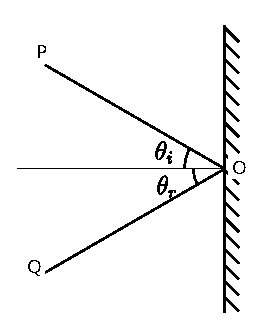
\includegraphics[width=\linewidth]{reflection_angles.pdf}
  \caption{Ángulos de reflexión}
  \label{fig:reflection_angles}
\end{wrapfigure}
La reflexión es el cambio en la dirección de propagación de una onda cuando choca contra una superficie y retorna al medio original.

Para ondas que inciden sobre una superficie lisa el ángulo de incidencia (\(\theta_i\)) es igual al ángulo de reflexión (\(\theta_r\)):
\[
  \theta_i = \theta_r
\]
Ejemplos:
\begin{itemize}
  \item Una onda en una cuerda que regresa al encontrar un extremo fijo.
  \item Un rayo de luz reflejándose en un espejo plano.
  \item Un eco producido por una onda sonora al rebotar en una pared.
\end{itemize}

\begin{wrapfigure}{l}{0.3\textwidth}
  \centering
  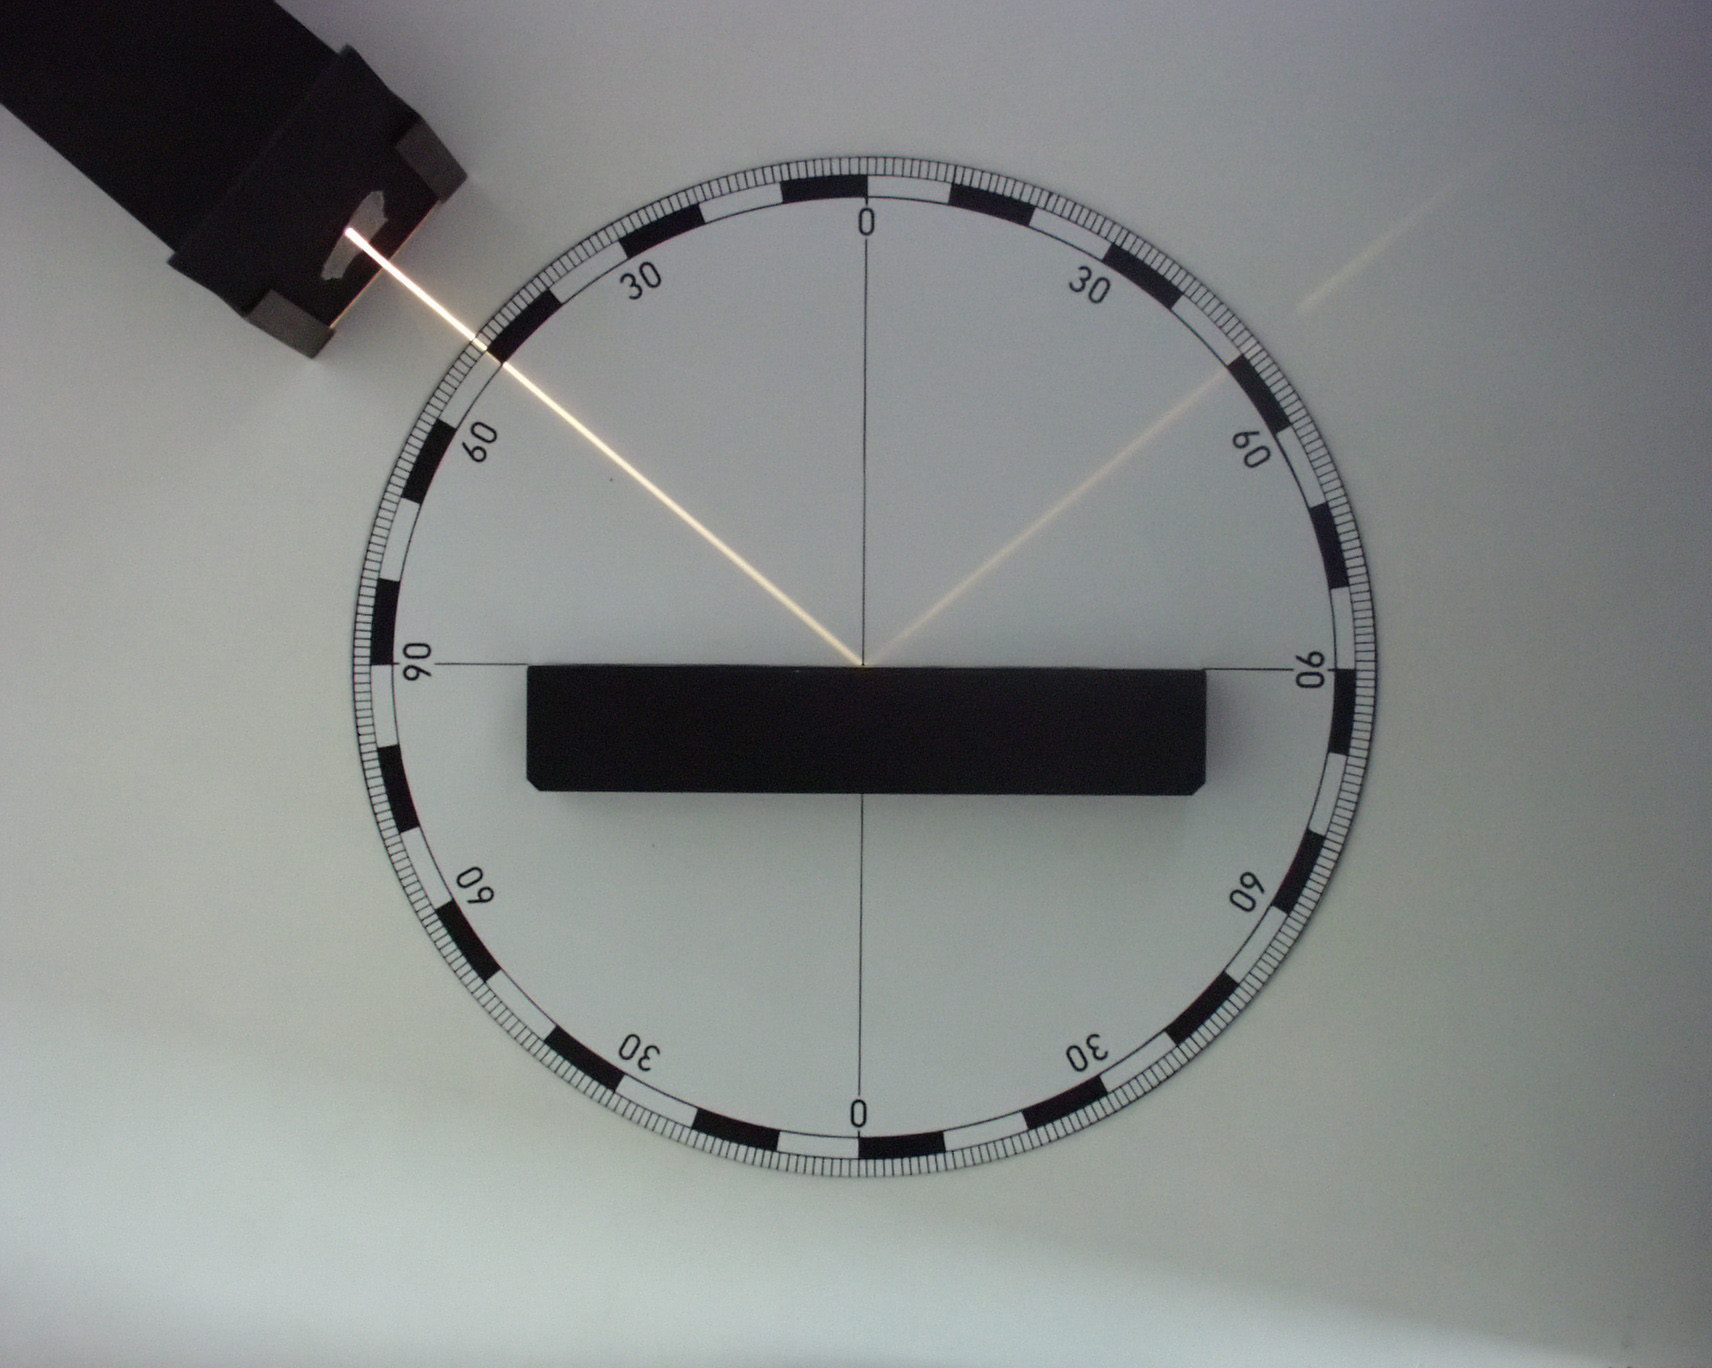
\includegraphics[width=\linewidth]{reflection_example.jpg}
  \caption{Reflexión de un haz de luz.}
  \label{fig:reflexion}
\end{wrapfigure}
En ondas mecánicas (como en cuerdas), la fase puede invertirse si la onda rebota en un medio más rígido (más denso). Se vió un ejemplo de esto con más detalle en la sección \ref{sec:waves_analisys}. 

En el caso de la luz (y en general cualquier onda electromagnética) también \textbf{puede invertir su fase} al reflejarse, dependiendo de las propiedades ópticas del medio en el que ocurre la reflexión.

La inversión de fase ocurre cuando una onda electromagnética se refleja en la superficie de \textbf{un medio con mayor índice de refracción que el medio del que proviene}. En ese caso, la onda reflejada experimenta un cambio de fase de \(\pi\) radianes (\(180^\circ\)).

En otras palabras, si la luz pasa de un medio con índice de refracción \(n_1\) a otro con \(n_2\), entonces:
\begin{itemize}
  \item Si \(n_2 > n_1\), la onda reflejada sufre un cambio de fase de \(\pi\) radianes (\(180^\circ\)).
  \item Si \(n_2 < n_1\), la onda reflejada no sufre un cambio de fase.
\end{itemize}

\subsubsection{Refracción y la ley de Snell}

La refracción es el fenómeno por el cual una onda electromagnética cambia de dirección y velocidad al pasar de un medio material a otro con diferente índice de refracción.

\begin{wrapfigure}{r}{0.3\textwidth}
  \centering
  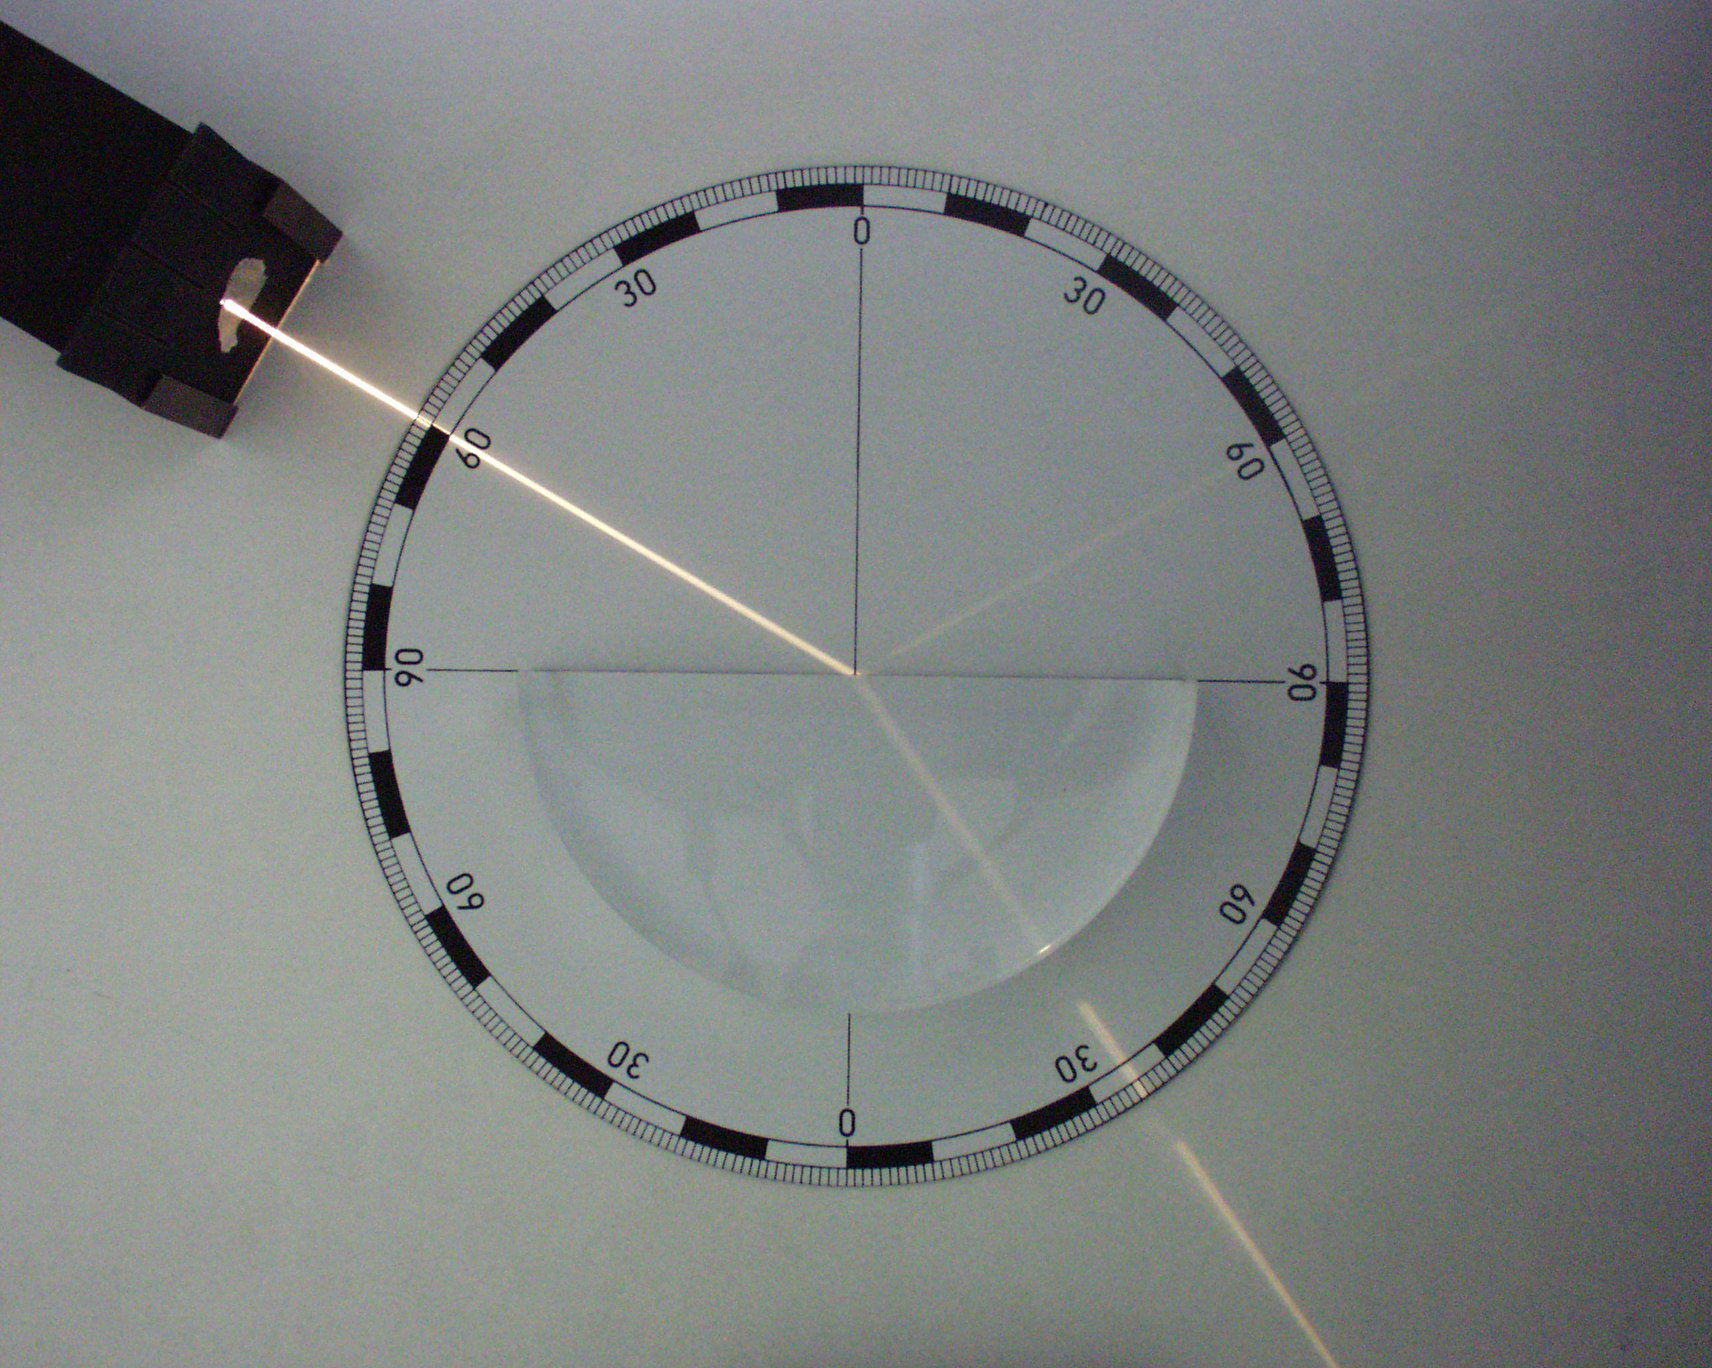
\includegraphics[width=\linewidth]{refraction_example.jpg}
  \caption{Refracción de un haz de luz.}
  \label{fig:refraction}
\end{wrapfigure}
Este cambio ocurre porque la velocidad de propagación de la onda no es la misma en distintos medios. Sin embargo, la frecuencia de la onda se conserva, lo cual implica que su longitud de onda cambia.

El índice de refracción \(n\) de un medio se define como:
\[
n = \frac{c}{v}
\]
donde:
\begin{itemize}
  \item \(c\) es la velocidad de la luz en el vacío.
  \item \(v\) es la velocidad de la onda en el medio.
\end{itemize}
Cuanto mayor es \(n\), más lento viaja la onda en ese medio.

\paragraph{Ley de Snell}

La dirección del rayo refractado está regida por la ley de Snell:
\[
n_1 \sin \theta_1 = n_2 \sin \theta_2
\]
donde:
\begin{itemize}
  \item \(n_1\), \(n_2\) son los índices de refracción de los medios 1 y 2.
  \item \(\theta_1\), \(\theta_2\) son los ángulos de incidencia y refracción medidos desde la normal a la superficie.
\end{itemize}

El límite o línea de separación entre los dos medios se llama frontera o interfaz.

\begin{figure}[ht]
  \centering
  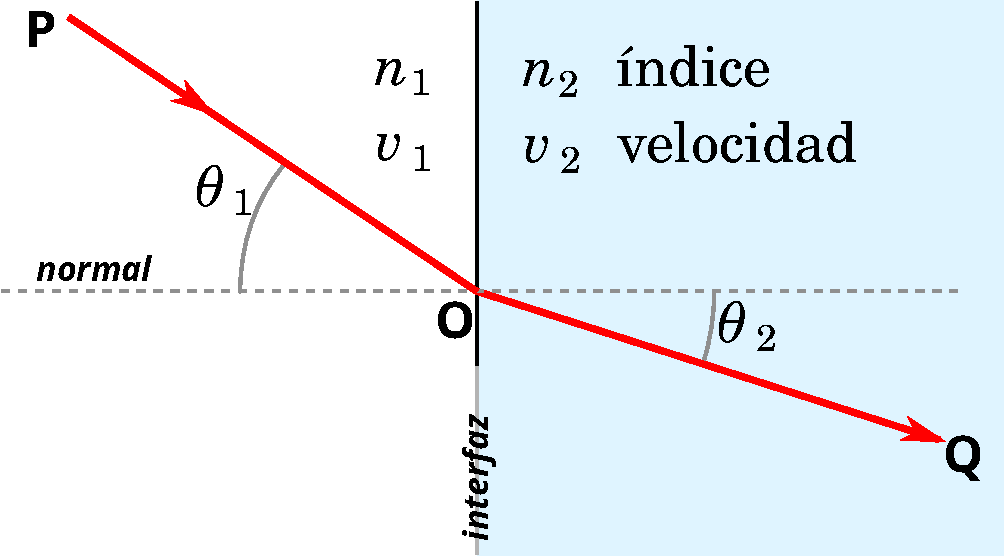
\includegraphics[width=0.5\textwidth]{snells_law.pdf}
  \caption{Ley de Snell.}
  \label{fig:snells_law}
\end{figure}

Cuando la onda cambia de medio la frecuencia \(f\) permanece constante (esto garantiza la continuidad temporal del campo eléctrico en la frontera), y la longitud de onda \(\lambda\) cambia según:
\[
\lambda_2 = \frac{v_2}{f} = \frac{c}{n_2 f}
\]
La dirección de propagación cambia si la onda incide oblicuamente.
\begin{itemize}
  \item Si \(n_2 > n_1\), la onda se desvía hacia la normal.
  \item Si \(n_2 < n_1\), se desvía lejos de la normal.
\end{itemize}
Sin embargo hay que tener en cuenta que existen casos especiales:
\begin{itemize}
  \item \textbf{Incidencia normal}: si la onda entra perpendicular a la superficie, no hay cambio de dirección, solo cambio en velocidad y longitud de onda.
  \item \textbf{Ángulo límite y reflexión total}: si la onda pasa de un medio más denso a uno menos denso y el ángulo de incidencia supera un cierto valor (ángulo crítico), no hay refracción, sino reflexión total interna.
\end{itemize}

\paragraph{Dispersion de la luz}

En términos simples, la \textbf{dispersión de la luz} es el fenómeno por el cual la luz blanca se separa en sus distintos colores (como los del arcoíris) cuando pasa a través de un material, como un prisma o gotas de agua.

Esto ocurre porque cada color de la luz viaja a una velocidad ligeramente diferente dentro del material, lo que provoca que se refracten en ángulos distintos. Los colores con menor longitud de onda, como el violeta o el azul, se desvían más que los de mayor longitud de onda, como el rojo.

\subsubsection{Interferencia}

La \textbf{interferencia} es un fenómeno característico de toda onda, y se refiere a la superposición de dos o más ondas coherentes que se encuentran en un mismo punto del espacio, generando un resultado que puede ser de mayor o menor intensidad, según la fase relativa entre ellas.

En el caso de ondas electromagnéticas, como la luz, la interferencia se manifiesta en variaciones de intensidad debidas a la superposición del campo eléctrico de las ondas.

Cuando dos ondas electromagnéticas se superponen, los campos eléctricos (\(\vec{E}\)) se suman vectorialmente (principio de superposición):
\[
\vec{E}_{\text{total}} = \vec{E}_1 + \vec{E}_2
\]
La intensidad observada es proporcional al cuadrado del campo eléctrico resultante:
\[
I \propto |\vec{E}_{\text{total}}|^2
\]
Esto puede generar dos situaciones:
\begin{enumerate}
  \item \textbf{Interferencia constructiva}: los campos eléctricos están en fase (máximos con máximos, mínimos con mínimos), y la intensidad aumenta.
  \item \textbf{Interferencia destructiva}: los campos están en oposición de fase (máximo con mínimo), y la intensidad disminuye o se anula.
\end{enumerate}

\paragraph{Condiciones necesarias para que haya interferencia observable}
\begin{itemize}
  \item Coherencia temporal: Las ondas deben tener frecuencias iguales o muy similares.
  \item Coherencia espacial: Las ondas deben mantener una diferencia de fase constante en el tiempo.
  \item Polarización compatible: Las componentes del campo eléctrico deben estar alineadas o parcialmente alineadas.
  \item Superposición espacial efectiva: Las ondas deben encontrarse en una región del espacio donde sus frentes de onda se crucen.
\end{itemize}

\paragraph{Diferencia de fase y camino óptico}

El camino óptico es una magnitud que permite cuantificar el efecto que tiene un medio sobre la propagación de una onda electromagnética, en particular sobre su fase. Se define como el producto del índice de refracción del medio y la distancia recorrida por la onda en ese medio.
\[
L = n \cdot d
\]
donde:
\begin{itemize}
  \item $L$ es el camino óptico,
  \item $n$ es el índice de refracción del medio,
  \item $d$ es la distancia física recorrida en el medio.
\end{itemize}
El camino óptico representa la distancia que la luz habría recorrido en el vacío durante el mismo tiempo que tarda en recorrer una distancia \(d\) en un medio con índice \(n\). Por eso, es útil para comparar fases entre ondas que han atravesado distintos medios. Dos ondas que recorren diferentes caminos ópticos pueden llegar con distinta fase al punto de interferencia, lo que afecta si la interferencia es constructiva o destructiva.

Cuando dos ondas recorren diferentes medios o longitudes, se habla de diferencia de camino óptico:
\[
\Delta L = n_1 d_1 - n_2 d_2
\]
Esta diferencia está directamente relacionada con la diferencia de fase:
\[
\Delta \varphi = \frac{2\pi}{\lambda_0} \Delta L
\]
donde \(\lambda_0\) es la longitud de onda en el vacío.

Entonces, retomando la ecuación de la interferencia, para que la interferencia sea observada, la diferencia de camino óptico \(\Delta L\) entre las ondas determina la diferencia de fase \(\Delta \varphi\) siendo:
\begin{itemize}
  \item Constructiva si \(\Delta L = m \lambda_0\), con \(m \in \mathbb{Z}\) (en fase (\(m\,2\pi\)))
  \item Destructiva si \(\Delta L = (m + 1/2)\lambda_0\) (en fase contraria (\(m\pi\)))
\end{itemize}
Algunos ejemplos típicos de interferencia son:
\begin{enumerate}
  \item Experimento de Young (doble rendija): produce franjas claras y oscuras por interferencia de la luz que pasa por dos rendijas muy cercanas.
  \item Interferencia en películas delgadas: como en burbujas de jabón o manchas de aceite, donde la luz se refleja en distintas capas.
\end{enumerate}

\begin{figure}[ht]
  \centering
  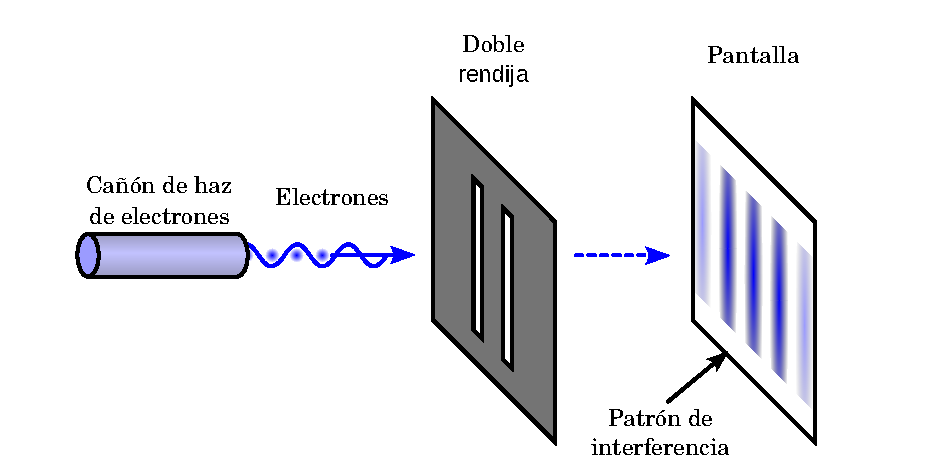
\includegraphics[width=0.65\textwidth]{double-slit.pdf}
  \caption{Interferencia de la luz por doble rendija}
  \label{fig:double_slit}
\end{figure}

\subsubsection{Difracción}

La difracción es la capacidad de una onda para rodear obstáculos o atravesar rendijas y luego extenderse en la región de sombra geométrica.

Factores relevantes:

\begin{itemize}
  \item Es más pronunciada si el tamaño de la rendija es comparable con la longitud de onda.
  \item A mayor longitud de onda, mayor difracción.
\end{itemize}

Ejemplos:

\begin{itemize}
  \item El sonido puede escucharse detrás de una pared aunque no haya línea de visión directa.
  \item Las ondas del mar rodean obstáculos como pilares o muelles.
\end{itemize}

\subsubsection{Polarización}

La polarización es la orientación de la vibración de una onda transversal en un solo plano. Solo ocurre con ondas transversales, como la luz; no ocurre con ondas longitudinales como el sonido.

Tipos de polarización:

\begin{itemize}
  \item Lineal: La onda vibra en un solo plano.
  \item Circular o elíptica: La dirección de vibración gira con el tiempo.
\end{itemize}

Métodos para polarizar la luz:

\begin{itemize}
  \item Filtros polarizadores (como en lentes de sol).
  \item Reflexión en ciertos ángulos (ángulo de Brewster).
  \item Dispersión (responsable del color azul del cielo).
\end{itemize}

Ejemplos:

\begin{itemize}
  \item Gafas de sol polarizadas que eliminan reflejos.
  \item Cristales líquidos en pantallas LCD utilizan luz polarizada.
\end{itemize}

